\section{Modello Relazionale}

Nel corso del tempo si sono sviluppati diversi modelli per la rappresentazione e l’organizzazione dei dati all’interno dei sistemi informativi. Tra i principali ricordiamo:

\begin{itemize}
    \item \textbf{Modello gerarchico/reticolare} (anni 1960–1970): tra i primi modelli di gestione dei dati, organizzati in forma gerarchica o a rete.
    \item \textbf{Modello relazionale} (anni 1980–oggi): introdotto da Edgar F. Codd, rappresenta i dati mediante tabelle (relazioni) e costituisce la base dei moderni DBMS relazionali.
    \item \textbf{Modello ad oggetti} (anni 1990–2000): integra i concetti di programmazione orientata agli oggetti con la gestione dei dati.
    \item \textbf{Modello a oggetti/relazionale (object–relational)} (anni 2000–oggi): un’evoluzione del modello relazionale che consente l’integrazione di tipi complessi, eredità e relazioni tra oggetti. Esempio: SQL3.
    \item \textbf{Modello a grafo – RDF (Resource Description Framework)} (anni 2005–oggi): rappresenta i dati sotto forma di grafo orientato, utile nel contesto del web semantico. Esempio: Neo4j.
    \item \textbf{Modelli noSQL} (document-based, column-based, key–value, ecc.) (anni 2010–oggi): nati per la gestione di grandi volumi di dati non strutturati e per garantire maggiore scalabilità. Esempio: MongoDB.
\end{itemize}
\subsection{Costrutti Principali del Modello Relazionale}
Il modello relazionale costituisce la base dei moderni database e si fonda su alcuni \textbf{costrutti principali}:

\begin{itemize}
    \item \textbf{Domini di base}: rappresentano l’insieme dei valori ammissibili per ciascun attributo.
    \item \textbf{Relazione (o tabella)}:
    \begin{itemize}
        \item Definizione come insieme di \textbf{n–uple} (righe).
        \item Ogni n–upla rappresenta un record all’interno della relazione.
    \end{itemize}
    \item \textbf{Superchiavi, Chiavi e Chiavi primarie}: identificano univocamente le tuple all’interno di una relazione.
    \item \textbf{Vincoli di integrità referenziale}: garantiscono la coerenza dei riferimenti tra tabelle.
    \item \textbf{Vincoli di integrità generici}: assicurano la validità logica dei dati rispetto a condizioni predefinite.
\end{itemize}
\subsection{Domini di Base}
Sono i domini da cui si scelgono i valori delle proprietà delle
istanze di informazione da rappresentare. I domini tipici sono:
\begin{itemize}
    \item Caratteri
    \item Stringhe
    \item Numeri
    \item Numeri decimali a virgola fissa
    \item Numeri decimali a virgola mobile
    \item Dominio del Tempo
\end{itemize}
\subsection{Costrutto Relazionale}
Una relazione può essere vista come una tabella ad esempio:

\begin{table}[H]
    \centering
    \renewcommand{\arraystretch}{1.2} % aumenta leggermente l'altezza delle righe
    \begin{tabular}{l c r}
        \hline
        \textbf{Città} & \textbf{CAP} & \textbf{Abitanti} \\
        \hline
        Milano  & 20100 & 1\,300\,000 \\
        Verona  & 37100 & 350\,000 \\
        Brescia & 25100 & 250\,000 \\
        \hline
    \end{tabular}
    \caption{Esempio di relazione \textbf{Città} con attributi \textit{(Nome, CAP, Abitanti)}}
    \label{tab:citta}
\end{table}
Una tabella è un contenitore di dati la cui struttura è caratterizzata da una lista di collonne:
\begin{itemize}
    \item I dati sono scritti nelle righe dove ogni riga descrive le
caratteristiche di un’istanza dell’informazione da rappresentare
    \item I valori contenuti nelle colonne descrivono sempre la stessa
proprietà delle istanze di informazione da rappresentare.
\end{itemize}
\subsubsection{Definizione: Relazione come insieme di ennuple (LISTS)}

Dati $n$ insiemi di valori (detti \textbf{domini}) $D_1, \ldots, D_n$ con $n > 0$, si indica con 
$D_1 \times \ldots \times D_n$ il loro \textbf{prodotto cartesiano}:

\[
D_1 \times \ldots \times D_n = 
\{ (v_1, \ldots, v_n) \mid v_1 \in D_1, \ldots, v_n \in D_n \}
\]

Una \textbf{relazione} $\rho$ di grado $n$ è un qualsiasi \textbf{sottoinsieme} di 
$D_1 \times \ldots \times D_n$:

\[
\rho \subseteq D_1 \times \ldots \times D_n
\]

dove $(v_1, \ldots, v_n)$ è una \textbf{ennupla} della relazione e 
$|\rho|$ rappresenta la \textbf{cardinalità} della relazione 
(ovvero il numero di ennuple presenti).
Si noti che i domini $D_1 ,\ldots,D_n$ possono essere a \textbf{cardinalità infinita}, mentre le relazioni sono SEMPRE a \textbf{cardinalità finita}.
Possiamo dire che
\begin{itemize}
    \item Non è definito alcun ordinamento sulle ennuple di una relazione
    \item Non sono ammessi DUPLICATI di una ennupla
    \item Nella definizione di relazione come insieme di ennuple, i valori nelle ennuple sono ordinati
\end{itemize}
\begin{figure}[H]
    \centering
    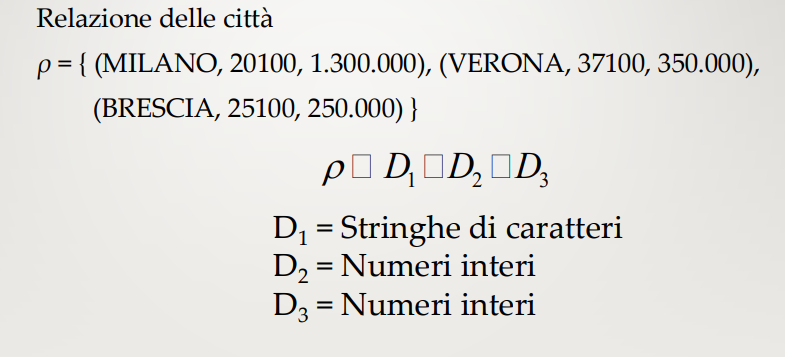
\includegraphics[width=0.75\linewidth]{image23.png}
    \caption{Esempio di relazione con insieme di ennuple}
\end{figure}
\paragraph{Accesso ai valori di una ennupla:}
Se $t$ e una ennupla $(V_1,\ldots,V_n)$ il valore posto in i-esima posizione si indica con la notazione $t[i]$. Questa modalità di accesso ai valori non è efficace per l'uso pratico delle relazioni.
Si preferisce quindi assegnare un nome alle colonne;ciò conduce all'introduzione della definizione come insieme di \textbf{TUPLE}.
\subsubsection{Definizione  RELAZIONE come insieme di tuple (MAPPINGS)}
Sia $X$ un insieme di nomi e si $\Delta$ l'insieme di tutti i domini di base ammessi dal modello.
Si definisce la funzione:\\
$DOM:X \to \Delta $\\

Tale funzione associa ad ogni nome A di X un dominio $DOM(A)$ di $\Delta$.I nomi di X si dicono \textbf{attributi}.
\begin{figure}[H]
    \centering
    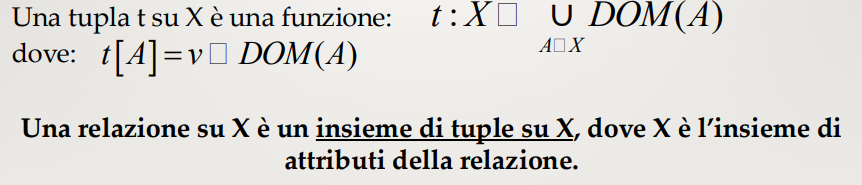
\includegraphics[width=0.75\linewidth]{image24.png}
\end{figure}
\begin{figure}[H]
    \centering
    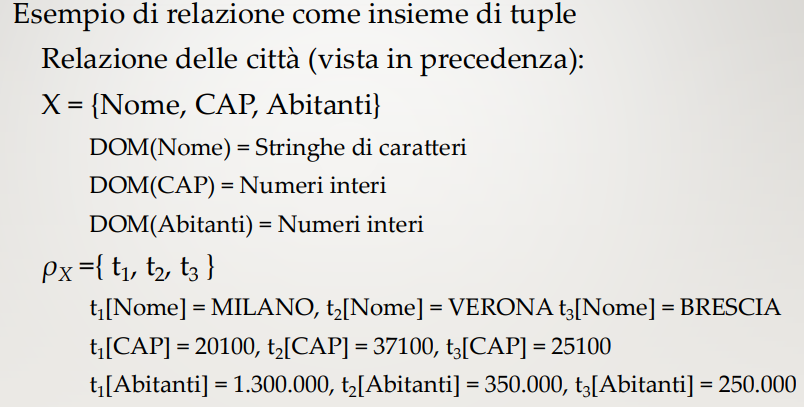
\includegraphics[width=0.75\linewidth]{image25.png}
    \caption{Esempio}
\end{figure}
\begin{itemize}
    \item Una relazione è un insieme di tuple e quindi non può contenere tuple duplicate
    \item I domini per gli attirbuti possono essere solo domini di base, non sono ammessi altri domini, ne il prodotto cartesiano di domini
    \item In generale una base di dati relazionale è costitutia da piu relazioni.
\end{itemize}
\subsection{Come progettare una basi di dati relazionale}
Nel modello relazionale lo schema è costituito da un insieme di relazioni o tabelle.
Lo strumento formale che serve per definire dipendenze tra attributi nel modello relazionale è costituito dalle \textbf{ dipendenze funzionali}.

\paragraph{Per Esempio:}
Vogliamo rappresentare in una base di dati relazionale le informazioni sulla proprietà degli appartamenti siti nel comune di Verona.
\begin{itemize}
    \item Per ogni appartamento volgiamo memorizzare : il codice ecografico (univoco), la categoria catastale e l'indirizzo composto da : via,numero civico, subalterno
    \item Per ogni proprietario si registra: il codice fiscale, il nome, il cognome e la data di nascita.
    \item Un appartamento può essere in comproprietà e un proprietario può possedere più appartamenti.
\end{itemize}
\begin{figure}[H]
    \centering
    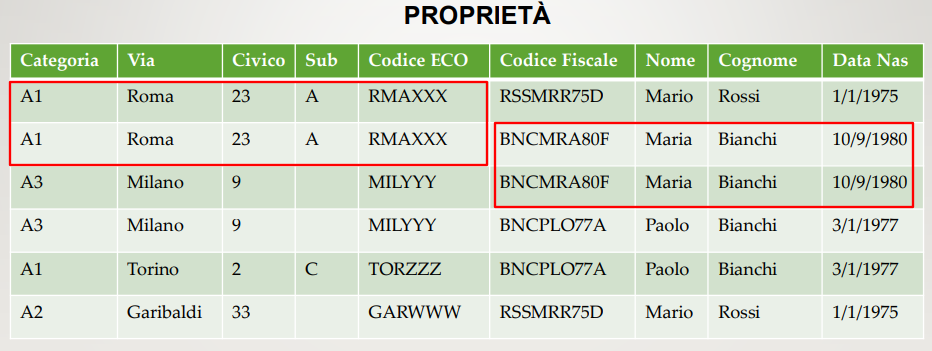
\includegraphics[width=0.75\linewidth]{image26.png}
    \caption{Schema relazionale con solo una relazione}
\end{figure}
Nella relazione unica ogni riga rappresenta un contratto di proprietà e richiede di precisare tutti i dati di un appartamento e tutti i dati di un proprietario.
Ciò implica che:
\begin{itemize}
    \item Non è possibile rappresentare un appartamento che non abbia un proprietario, né rappresentare un proprietario senza appartamento,
    \item I dati di un appartamento vengono replicati per ogni proprietario
    \item I dati di un proprietario vengono replicati per ogni appartamento di proprietà.
\end{itemize}
\paragraph{Anomalie:} La presenza di ridondanza inutile nella base di dati provoca le seguenti anomalie:
\begin{itemize}
    \item \textbf{ANOMALIE DI AGGIORNAMENTO} : per aggiornare il valore di un attributo si è obbligati a modificare tale valore su più tuple.
    \item  \textbf{ANOMALIE DI INSERIMENTO} : per inserire una nuova tupla è necessario inserire valori al momento sconosciuti (sostituibili da valori nulli) per gli attributi non disponibili.
    \item \textbf{ANOMALIE DI CANCELLAZIONE} : per cancellare una tupla è necessario cancellare valori ancora validi oppure inserire valori nulli per gli attributi da cancellare.
\end{itemize}
E possibile ridurre la ridondanza nei dati decomponendo la relazione. Sono possibili diverse decomposizioni.
\begin{figure}[H]
    \centering
    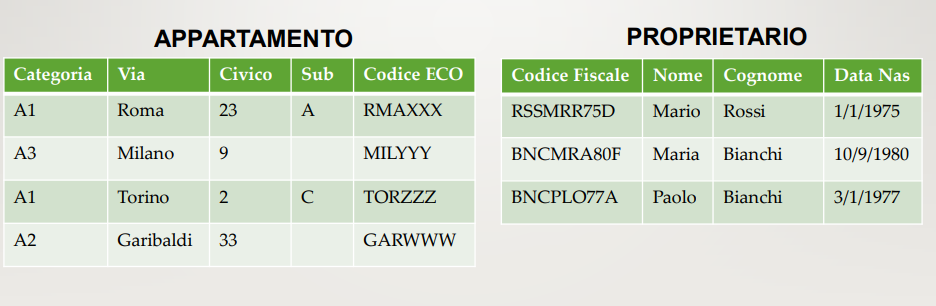
\includegraphics[width=0.75\linewidth]{image27.png}
    \caption{Decomposizione 1}
\end{figure}
\begin{figure}[H]
    \centering
    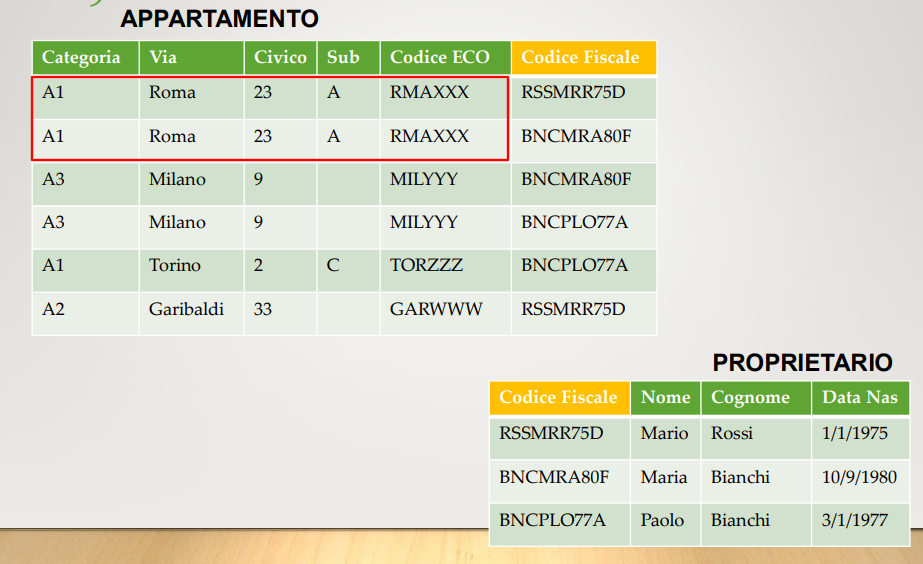
\includegraphics[width=0.75\linewidth]{image28.png}
    \caption{Decomposizione 2}
    \label{fig:placeholder}
\end{figure}
\begin{figure}[H]
    \centering
    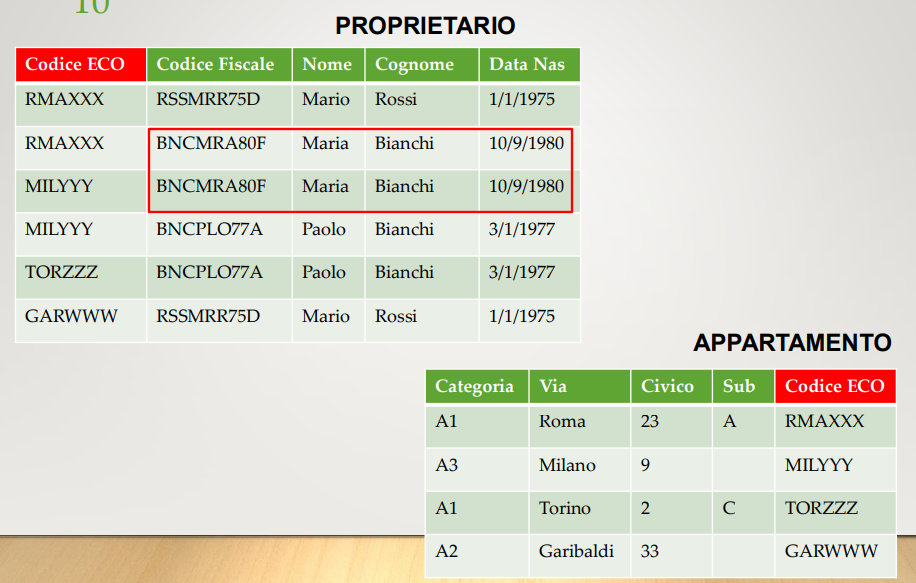
\includegraphics[width=0.75\linewidth]{image29.png}
    \caption{Decomposizione 3}
\end{figure}
\begin{figure}[H]
    \centering
    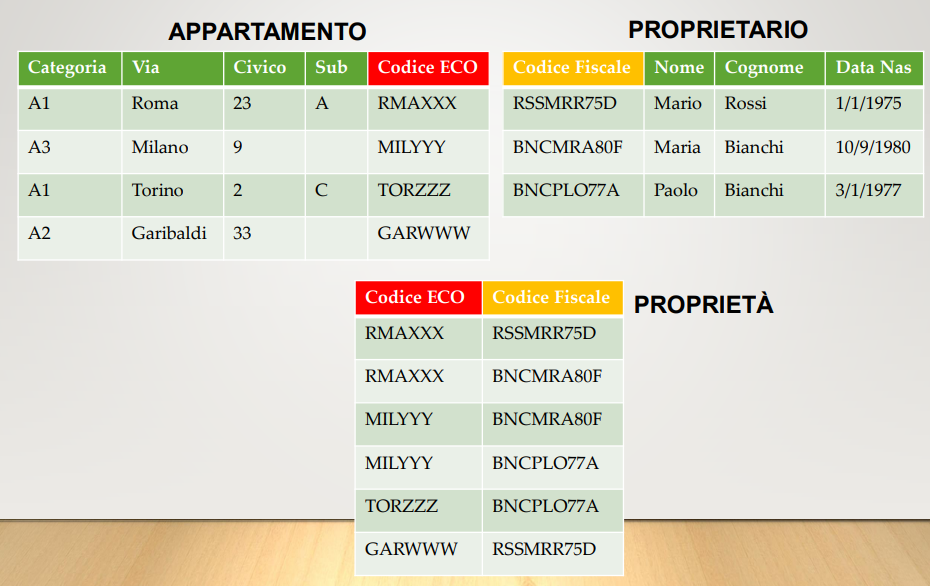
\includegraphics[width=0.75\linewidth]{image30.png}
    \caption{Decomposizione 4}
\end{figure}
Si noti che i legami tra relazioni si realizzano attraverso la replicazione di un insieme di attributi, dove il legame tra due tuple si intende stabilito quando esse presentano gli stessi valori negli attributi replicati.
Il modello relazionale è \textbf{value-based} (basato su valori).
Il modello non prevede l'uso di puntatori per rappresentare legami tra i dati.
Essere value-based implica:
\begin{itemize}
    \item Completa indipendenza dall'implementazione e dallo schema fisico
    \item Facilità di trasferimento dei dati tra sistemi
    \item Viene rappresentato solo ciò che è rilevante per il sistema informativo
\end{itemize}
\subsubsection{Terminologia di schema di una relazione}
E costituito dal nome della relazione e da un insieme di nomi per i suoi attributi:\\
$R(X)$ oppure $R(A_1,\dots,A_n)$ oppure $R(A_1:D_1,\dots,A_n:D_n)$
\subsubsection{Terminologia Schema di una base di dati}
E costituito da un insieme di schemi di relazioni:\\
$S = \{R_1(X_1),\dots,R_n(X_n)\}$ con $R_1 \neq R_2 \neq \dots R_n$
\subsubsection{Terminologia istanza di una relazione di schema $R(X)$}
E un insieme r di tuple su X dove $r = \{ t_1,\dots,t_k \}$
\subsubsection{Terminologia istanza di una base di dati di schema $S = \{R_1(X_1),\dots,R_n(X_n)$}
E costituito da un insieme di istanze delle relazioni $R_1(X_1),\dots,R_n(X_n): db = \{r_1,\dots,r_n\}$
\subsection{Valori nulli}

Secondo la definizione formale di \textit{relazione}, ogni tupla dovrebbe contenere per ciascun attributo un valore appartenente al relativo dominio.  
Nelle basi di dati reali, però, questa condizione non è sempre rispettabile: può accadere che un attributo non abbia un valore disponibile.  

I motivi principali per cui un valore può mancare sono i seguenti:

\begin{itemize}
    \item \textbf{Valore inesistente}  
    L'attributo $A$ è concettualmente opzionale: per quella specifica istanza non esiste alcun valore significativo da inserire.  
    \textit{Esempio:} il campo ``secondo numero di telefono'' per un cliente che possiede un solo numero.

    \item \textbf{Valore sconosciuto}  
    Il valore dell'attributo $A$ esiste, ma non è attualmente noto alla base di dati.  
    \textit{Esempio:} l'indirizzo e-mail di un utente appena registrato che non lo ha ancora comunicato.

    \item \textbf{Valore sconosciuto o inesistente}  
    Non è possibile stabilire se l'informazione manchi perché non esiste o perché non è ancora conosciuta, oppure si preferisce rappresentare entrambe le situazioni allo stesso modo.  
    \textit{Esempio:} il campo ``data di scadenza del contratto'', che potrebbe non essere ancora stata definita oppure semplicemente non comunicata.
\end{itemize}
Per gestire queste situazioni si introduce il \textbf{valore nullo}.  
In questo modo il valore di un attributo in una tupla può essere:
\begin{itemize}
    \item un valore appartenente al dominio dell'attributo;
    \item il \texttt{NULL}, utilizzato per rappresentare un'informazione assente (inesistente o sconosciuta).
\end{itemize}

\textit{Esempio:} nel campo ``numero di telefono fisso'' di una tabella dei clienti, un cliente che non possiede un telefono fisso avrà come valore \texttt{NULL}.
\begin{figure}[H]
    \centering
    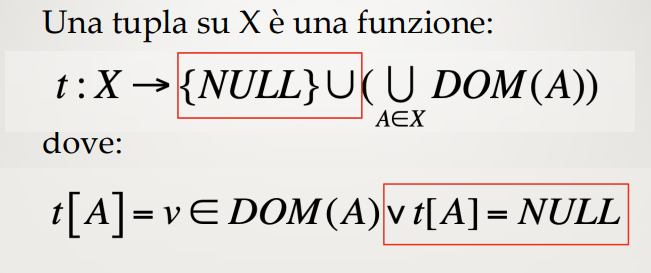
\includegraphics[width=0.75\linewidth]{image31.png}
    \caption{Tupla su X con valori nulli}
\end{figure}
Si noti che:

\begin{itemize}
    \item \textbf{La presenza di valori nulli è ammessa solo in alcuni attributi.}  
    Non è infatti possibile avere tuple composte esclusivamente da valori nulli, poiché non rappresenterebbero alcuna informazione utile.

    \item \textbf{I valori nulli possono creare problemi negli attributi usati per rappresentare legami tra tuple.}  
    In particolare, negli attributi che fungono da chiave esterna, un valore \texttt{NULL} potrebbe rendere impossibile stabilire la relazione con altre tuple.
\end{itemize}

\textit{Esempio:}  
Si consideri una tabella \texttt{Prenotazioni} con l'attributo \texttt{idCliente} come chiave esterna verso la tabella \texttt{Clienti}.  
Se \texttt{idCliente} fosse \texttt{NULL}, non sarebbe possibile sapere quale cliente ha effettuato la prenotazione, rendendo l'informazione inutilizzabile.
\subsection{Vincoli di integrità}
Spesso è necessario introdurre dei \textbf{vincoli} (restrizioni) sull'istanza
di una base di dati, poiché non tutte le configurazioni possibili sono
compatibili con il sistema informativo che si vuole rappresentare.

Per specificare quali istanze sono considerate corrette si introduce il
concetto di \textbf{vincolo di integrità}.

\begin{tcolorbox}[
colback=yellow!20,
colframe=yellow!50!black,
title=\textbf{Vincolo di Integrità}
]
Un \textbf{vincolo di integrità} è una condizione (espressa come un predicato)
che deve essere sempre verificata da ogni istanza della base di dati.  
I vincoli di integrità assicurano che i dati memorizzati siano consistenti,
coerenti e validi rispetto al modello del sistema informativo.
\end{tcolorbox}
\subsection{Esempi di vincoli}

Siano date le seguenti relazioni:

\begin{itemize}
    \item \texttt{TRENO(Numero, OraPart, MinutoPart, Categoria, Destinazione, OraArr, MinutoArr)}
    \item \texttt{FERMATA(NumTreno, Stazione, OraFer, MinutoFer)}
\end{itemize}

I seguenti predicati esprimono possibili \textbf{vincoli di integrità} sulla relazione \texttt{TRENO}:

\[
\forall t \in TRENO :\; t[\text{OraPart}] \in \{0,1,\ldots,23\}
\]

\[
\forall t \in TRENO :\; t[\text{MinutoPart}] \in \{0,1,\ldots,59\}
\]

\[
\forall t \in TRENO :\; t[\text{Numero}] > 0
\]

\[
\forall t \in TRENO :\; t[\text{Numero}] > 5000 \;\Rightarrow\; t[\text{Categoria}] = \text{'regionale'}
\]
\[
\forall t, t' \in TRENO :\; t \neq t' \;\Rightarrow\; t[\text{Numero}] \neq t'[\text{Numero}]
\]
\textit{(Vincolo di unicità sul Numero del treno)}

\[
\forall f \in FERMATA :\; \exists t \in TRENO :\; t[\text{Numero}] = f[\text{NumTreno}]
\]
\textit{(Vincolo di chiave esterna: ogni fermata deve riferirsi a un treno esistente)}

\[
\forall t \in TRENO :\; t[\text{Categoria}] = \text{'regionale'}
\Rightarrow \exists f \in FERMATA :\; f[\text{NumTreno}] = t[\text{Numero}]
\]
\textit{(Se un treno è regionale allora deve avere almeno una fermata)}
\subsection{Classificazione vincoli di integrità}
Si distinguono inoltre alcuni vincoli particolari che rivestono un ruolo 
fondamentale, poiché assicurano proprietà generali valide per tutti gli 
schemi relazionali. Tali vincoli sono detti \textbf{vincoli strutturali}.

Essi comprendono:

\begin{itemize}
    \item \textbf{Vincoli di dominio}  
    Specificano quali valori possono essere assegnati a ciascun attributo 
    (esempio: l’attributo \texttt{OraPart} deve essere compreso tra 0 e 23).

    \item \textbf{Vincoli di tupla}  
    Impongono condizioni che devono essere verificate all'interno di una 
    singola tupla (esempio: \texttt{Numero} > 0).

    \item \textbf{Vincoli intrarelazionali}  
I vincoli intrarelazionali impongono condizioni sul contenuto di una
relazione e richiedono che ogni tupla soddisfi una certa proprietà
rispetto alle altre tuple della stessa relazione.

Una categoria particolarmente rilevante di tali vincoli è costituita
dai \textbf{vincoli di chiave}, che comprendono:
\begin{itemize}
    \item \textbf{Superchiave}: Data una relazione di schema $R(X)$, un insieme di attributi $K \subseteq X$
è una \textbf{superchiave} per $R(X)$ se, per ogni istanza $r$ di $R(X)$,
vale la seguente condizione:

\[
\forall t, t' \in r : t \neq t' \;\Rightarrow\; t[K] \neq t'[K]
\]

dove:

\[
t[K] \neq t'[K] \;\equiv\; \exists A_i \in K : t[A_i] \neq t'[A_i]
\]

    \item \textbf{Chiave candidata} : Data una relazione di schema $R(X)$, un insieme di attributi $K$, 
sottoinsieme di $X$, è \textbf{chiave candidata} (o \textbf{chiave}) per $R(X)$
se $K$ è superchiave per $R(X)$ e vale la seguente condizione:

\[
\neg \exists K' \subset K : K' \text{ è superchiave per } R(X)
\]
    \item \textbf{Chiave primaria} : Data una relazione di schema $R(X)$, la sua \textbf{chiave primaria}
è la chiave candidata scelta per \textit{identificare le tuple della relazione}.

Una chiave primaria $K$ ha le seguenti caratteristiche:

\begin{itemize}
    \item Non contiene \underline{mai valori nulli}.
    \item Su $K$ il sistema genera una struttura d’accesso ai dati (o indice)
          per supportare le interrogazioni.
\end{itemize}
\begin{tcolorbox}[colback=yellow!20, colframe=yellow!50!black, title={Kristian semplifica così – Le tre chiavi spiegate intuitivamente}]

\textbf{Superchiave}  
Una superchiave è \textbf{qualsiasi insieme di attributi che distingue sempre le tuple}.  
Se due tuple sono diverse, almeno un attributo della superchiave è diverso.

\textbf{Esempio:}  
Nella tabella STUDENTI(\underline{Matricola}, Nome, Cognome, Email)  
- Insiemi come \{Matricola\}, \{Matricola, Nome\}, \{Email, Cognome\} sono tutte superchiavi.  
Perché? Perché non esistono due studenti con la stessa combinazione di quei valori.

\vspace{0.4cm}

\textbf{Chiave candidata}  
Una chiave candidata è una \textbf{superchiave minimale}:  
non puoi togliere nessun attributo senza perdere l’unicità.

\textbf{Esempio:}  
- \{Matricola\} è chiave candidata perché basta da sola.  
- \{Email\} è un’altra chiave candidata.  
- Ma \{Matricola, Nome\} \textbf{non} è candidata: contiene attributi inutili, è troppo “larga”.

\vspace{0.4cm}

\textbf{Chiave primaria}  
È la \textbf{chiave candidata scelta} per identificare ufficialmente le tuple.  
Non può contenere NULL e il DB crea un indice su di essa.

\textbf{Esempio:}  
Se in STUDENTI scegliamo la chiave candidata \{Matricola\}, quella diventa la chiave primaria.  
Serve per identificare uno studente, fare ricerche, creare collegamenti con altre tabelle.

\end{tcolorbox}

\end{itemize}

 
    \item \textbf{Vincoli interrelazionali}  
    I vincoli interrelazionali impongono una restrizione al contenuto di una relazione
e specificano una condizione che ogni tupla della relazione deve soddisfare
rispetto alle tuple di altre relazioni della base di dati.Una sottocategoria importante di tali vincoli è costituita dai:
    \begin{itemize}
        \item \textbf{Vincoli di integrità referenziale}  
impone che ogni valore di una
\textit{chiave esterna} (foreign key) presente in una relazione
debba necessariamente comparire come valore di \textit{chiave primaria}
(primary key) nella relazione a cui fa riferimento.
%
In questo modo si garantisce la coerenza dei dati tra più tabelle
e si impedisce l'inserimento di tuple ``orfane'' non collegate a dati esistenti.

\begin{tcolorbox}[
colback=yellow!15!white,
colframe=orange!80!black,
title=\textbf{Kristian semplifica in questo modo}
]
Il vincolo di integrità referenziale è una regola che assicura che due tabelle
rimangano sempre coerenti tra loro.

\textbf{Significa:} se in una tabella inserisco una \textit{chiave esterna},
quel valore deve esistere come \textit{chiave primaria} nella tabella collegata.

\textbf{Esempio intuitivo:}

\begin{itemize}
    \item Tabella \texttt{Studenti(id, nome)}
    \item Tabella \texttt{Esami(idStudente, voto)}
\end{itemize}

Nella tabella \texttt{Esami}, il campo \texttt{idStudente} è una \textbf{foreign key}:
può contenere solo valori che esistono come \texttt{id} nella tabella \texttt{Studenti}.

Se provo a inserire un esame per lo studente \texttt{id = 50}, ma nella tabella
\texttt{Studenti} non esiste lo studente 50, il database blocca l'inserimento
perché violerei il vincolo di integrità referenziale.
\end{tcolorbox}
    \end{itemize}
\end{itemize}
\subsection{Notazione per indicare i vincoli strutturali}

\subsubsection{Chiave primaria}

La chiave primaria di una relazione $R(X)$ viene indicata
\textbf{sottolineando gli attributi} che la compongono.

Supponiamo che, per la tabella \texttt{TRENO}, venga scelto come chiave primaria
l'attributo \texttt{Numero}.  
La notazione per indicare tale chiave è:

\[
\texttt{TRENO(}\underline{\texttt{Numero}}\texttt{, OraPart, MinutoPart, Categoria, Destinazione, OraArr, MinutoArr)}
\]

Per la tabella \texttt{FERMATA}, la chiave primaria è composta dagli attributi
\texttt{NumTreno}, \texttt{Stazione}, \texttt{OraFer} e \texttt{MinutoFer}.
Si indica così:

\[
\texttt{FERMATA(}\underline{\texttt{NumTreno, Stazione}}\texttt{, OraFer, MinutoFer)}
\]

\bigskip

\subsubsection{Vincolo di integrità referenziale}

Un \textbf{vincolo di integrità referenziale} viene indicato
\textbf{riquadrando gli attributi soggetti al vincolo}
(nella tabella figlia)  
e collegandoli con una freccia al riquadro degli attributi
della tabella da cui la chiave primaria proviene (tabella padre).

Supponiamo che nella tabella \texttt{FERMATA} l'attributo
\texttt{NumTreno} sia una chiave esterna che fa riferimento
alla chiave primaria \texttt{Numero} della tabella \texttt{TRENO}.

La notazione diventa:

\[
\boxed{\texttt{Numero}} \quad \longleftarrow \quad
\texttt{TRENO(}\underline{\texttt{Numero}}\texttt{, OraPart, MinutoPart, Categoria, Destinazione, OraArr, MinutoArr)}
\]

\vspace{0.3cm}

\[
\boxed{\texttt{NumTreno}} \quad
\texttt{FERMATA(}\underline{\texttt{NumTreno, Stazione}}\texttt{, OraFer, MinutoFer)}
\]

\bigskip

\begin{tcolorbox}[
colback=yellow!15!white,
colframe=orange!80!black,
title=\textbf{Kristian semplifica in questo modo}
]
\textbf{Chiave primaria}: sottolineo gli attributi che identificano univocamente
le tuple della tabella.

\textbf{Chiave esterna (integrità referenziale)}: metto un riquadro attorno
all'attributo nella tabella ``figlia'' e lo collego con una freccia
alla chiave primaria della tabella ``padre''.

In questo modo si vede subito da dove arriva il valore e quale tabella controlla
la sua validità.
\end{tcolorbox}
\subsection{Esercizio}
\begin{figure}[H]
    \centering
    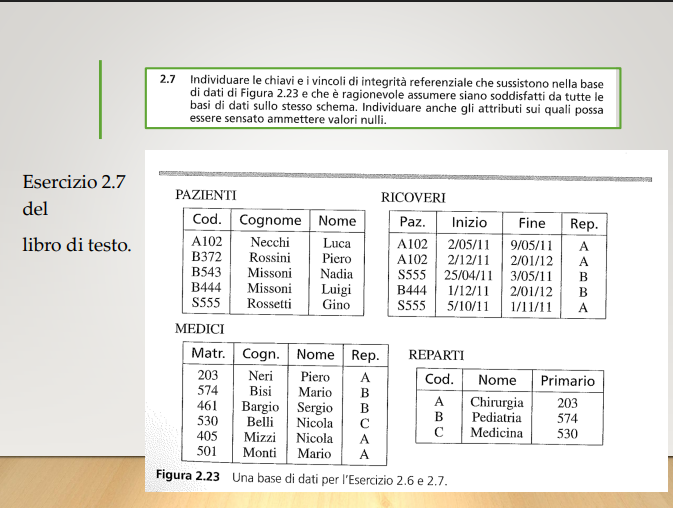
\includegraphics[width=1\linewidth]{image32.png}
    \label{fig:placeholder}
\end{figure}
\begin{figure}[H]
    \centering
    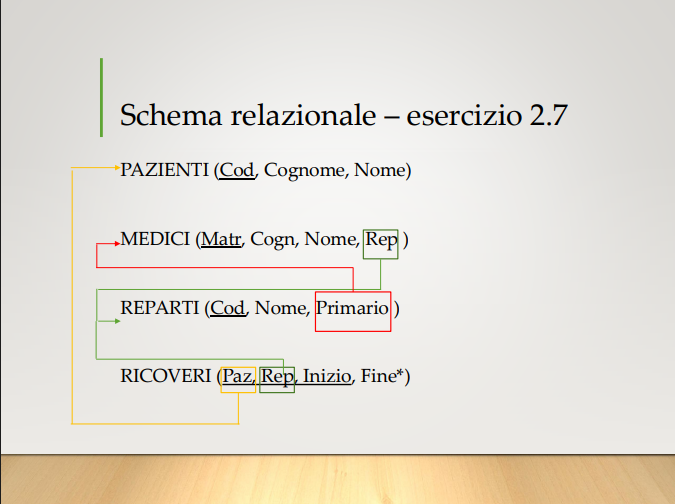
\includegraphics[width=1\linewidth]{image33.png}
    \caption{Soluzione}
    \label{fig:placeholder}
\end{figure}
\subsection{Progettazione Logica}

L’obiettivo della progettazione logica è quello di produrre uno \textbf{schema logico} che rappresenti in modo corretto, completo ed efficace tutte le informazioni contenute nello \textbf{schema concettuale}.

Prima della traduzione può essere necessario \textbf{ristrutturare lo schema ER} per i seguenti motivi:
\begin{itemize}
    \item \textbf{Semplificare} la fase di traduzione verso il modello logico.
    \item \textbf{Ottimizzare} le strutture in base al \textit{carico di lavoro} previsto (operazioni e query più frequenti).
\end{itemize}

Le principali fasi della \textbf{ristrutturazione dello schema ER} sono:
\begin{itemize}
    \item Analisi delle \textbf{ridondanze} dovute alla presenza di dati derivabili.
    \item \textbf{Eliminazione delle generalizzazioni} tramite le diverse strategie di trasformazione.
    \item \textbf{Accorpamento} o \textbf{partizionamento} di entità e relazioni, quando necessario.
    \item Scelta degli \textbf{identificatori principali} più adatti ed efficienti.
\end{itemize}

\subsubsection{Analisi della derivabilità}

L’analisi della derivabilità serve a individuare \textbf{dati che possono essere ricavati (derivati) da altri dati già presenti nello schema}.  
Questi dati non vanno memorizzati perché occupano spazio inutilmente e possono creare inconsistenze.

Esempi di dati derivabili:
\begin{itemize}
    \item \textbf{Attributi calcolabili} a partire da altri attributi della stessa entità  
    (es. ``età'' derivabile dalla ``data di nascita'').
    
    \item \textbf{Attributi derivabili} da informazioni presenti in entità diverse  
    (es. ``numero totale degli ordini di un cliente'' ricavabile dalla relazione \textit{Ordini}).
    
    \item \textbf{Attributi ottenuti con un conteggio}  
    (es. ``numero di iscritti a un corso'' ricavabile contando le partecipazioni).
    
    \item \textbf{Relazioni derivabili} dalla combinazione di altre relazioni  
    (es. una relazione ``LavoraIn'' può essere derivata combinando ``Impiegato'' e ``Dipartimento'' tramite una relazione intermedia).
\end{itemize}
\subsubsection{Analisi delle ridondanze}

In questa fase vengono analizzati i \textbf{dati derivabili} per decidere se conviene:
\begin{itemize}
    \item \textbf{Memorizzare il dato derivabile}, quando il costo del calcolo è \emph{maggiore} del costo di aggiornamento.
    \item \textbf{Non memorizzarlo e calcolarlo quando serve}, quando il costo del calcolo è \emph{minore} del costo di aggiornamento.
\end{itemize}

Il \textbf{costo} viene misurato in termini di numero di accessi per unità di tempo, valutando:
\begin{itemize}
    \item la frequenza con cui il dato deve essere calcolato,
    \item la frequenza con cui il dato dovrebbe essere aggiornato.
\end{itemize}
\subsubsection{Eliminazione delle Generalizzazioni}

Nel modello relazionale le generalizzazioni non sono direttamente rappresentabili.  
Per questo motivo esistono tre possibili strategie per trasformarle:
\begin{itemize}
    \item \textbf{Accorpamento delle entità figlie nel padre}.
    \item \textbf{Accorpamento dell’entità padre nelle entità figlie}.
    \item \textbf{Sostituzione della generalizzazione con relazioni}.
\end{itemize}

\subsubsection{Accorpamento delle entità figlie nel padre} 
Questa soluzione prevede:
\begin{itemize}
    \item Eliminazione delle entità figlie.
    \item Trasferimento nel padre di tutti gli attributi specifici delle entità figlie, trattandoli come \textbf{attributi opzionali}.
    \item Accorpamento nel padre di tutte le relazioni che coinvolgevano le entità figlie, impostando la \textbf{cardinalità minima a 0} dal lato del padre.
    \item Aggiunta di un attributo \textbf{TIPO} per distinguere le occorrenze corrispondenti alle ex entità figlie.
\end{itemize}
\begin{figure}[H]
    \centering
    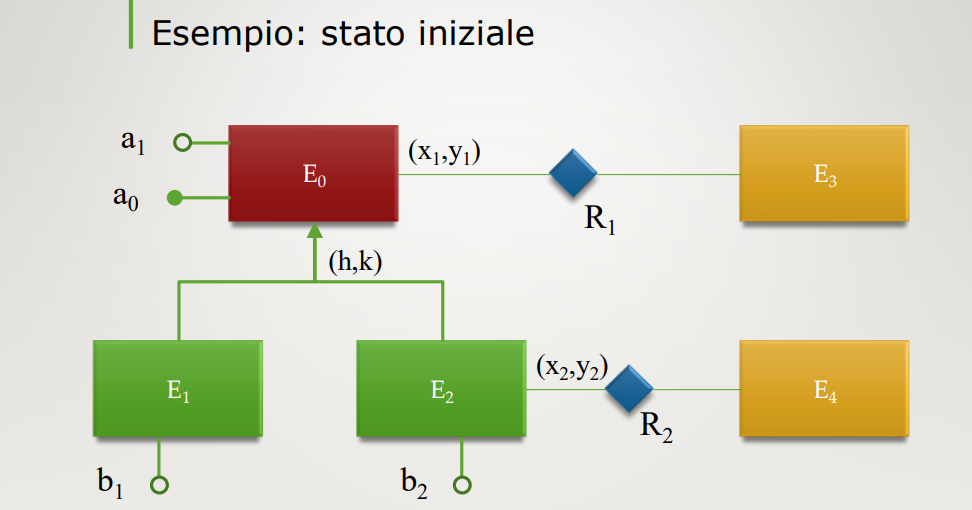
\includegraphics[width=1\linewidth]{image34.png}
    \caption{Stato iniziale}
\end{figure}
\begin{figure}[H]
    \centering
    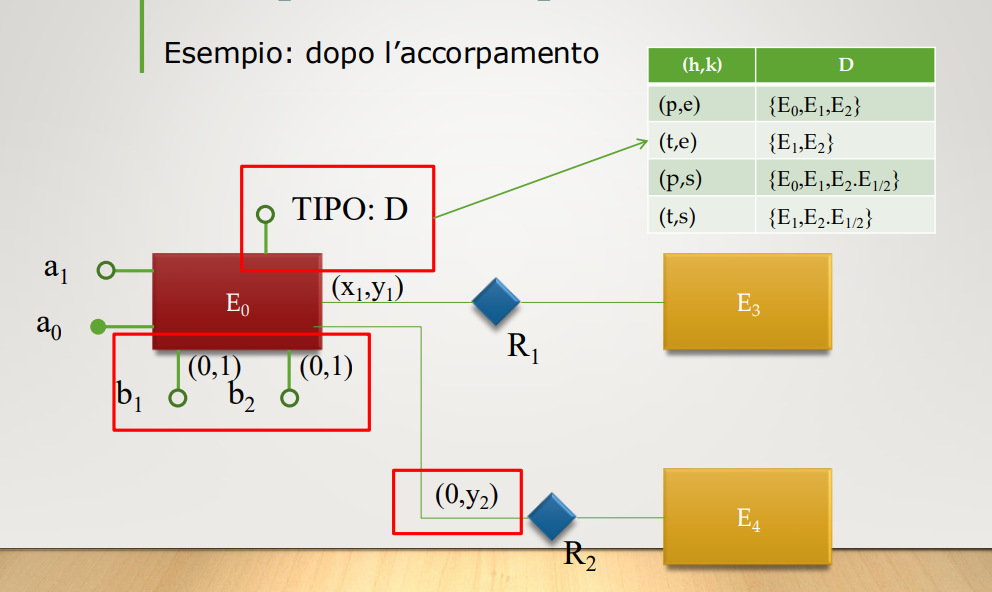
\includegraphics[width=1\linewidth]{image35.png}
    \caption{Accorpamento delle entità figlie nel padre}
\end{figure}
\subsubsection{Accorpamento del padre nelle entità figlie}

Questa trasformazione può essere applicata solo quando la generalizzazione è \textbf{totale}.  
La procedura consiste nei seguenti passi:
\begin{itemize}
    \item Eliminazione dell’entità padre.
    \item Replicazione degli attributi dell’entità padre in ciascuna entità figlia.
    \item Partizionamento, tra le entità figlie, delle relazioni che coinvolgevano l’entità padre, assegnando \textbf{cardinalità minima pari a 0} dal lato delle entità esterne.
\end{itemize}

\begin{figure}[H]
    \centering
    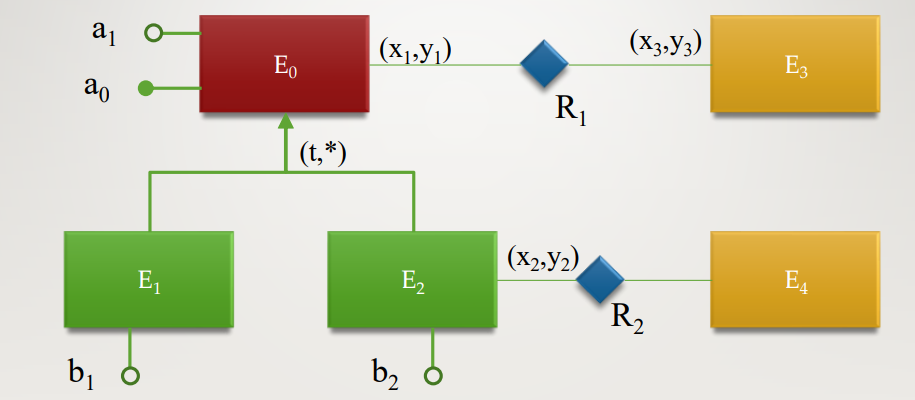
\includegraphics[width=1\linewidth]{image36.png}
    \caption{Schema iniziale}
\end{figure}

\begin{figure}[H]
    \centering
    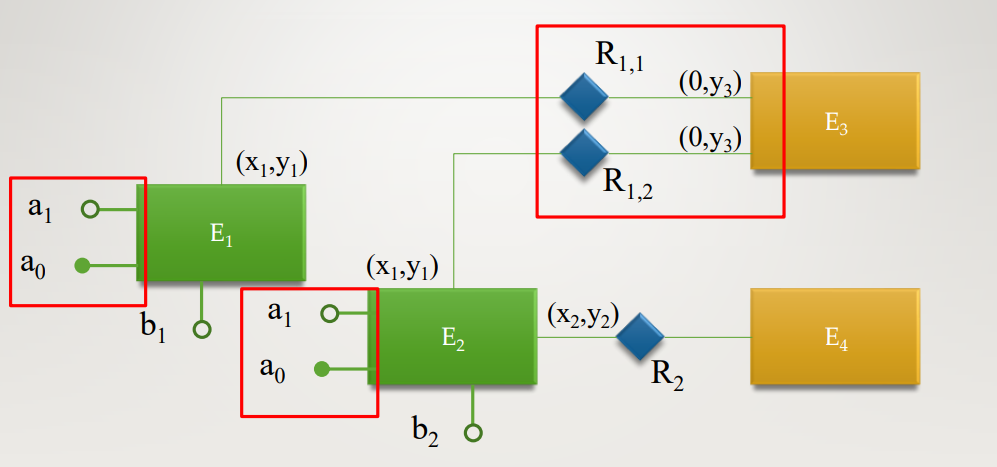
\includegraphics[width=1\linewidth]{image37.png}
    \caption{Accorpamento nelle entità figlie}
\end{figure}
\subsubsection{Sostituzione con relazioni}

Questa strategia sostituisce la generalizzazione con un insieme di relazioni esplicite.  
I passi da seguire sono:
\begin{itemize}
    \item Eliminazione della generalizzazione.
    \item Inserimento di $n$ relazioni tra l’entità padre e ciascuna delle $n$ entità figlie.
    \item Mantenimento degli attributi nelle entità in cui si trovavano originalmente, senza spostamenti.
\end{itemize}

\begin{figure}[H]
    \centering
    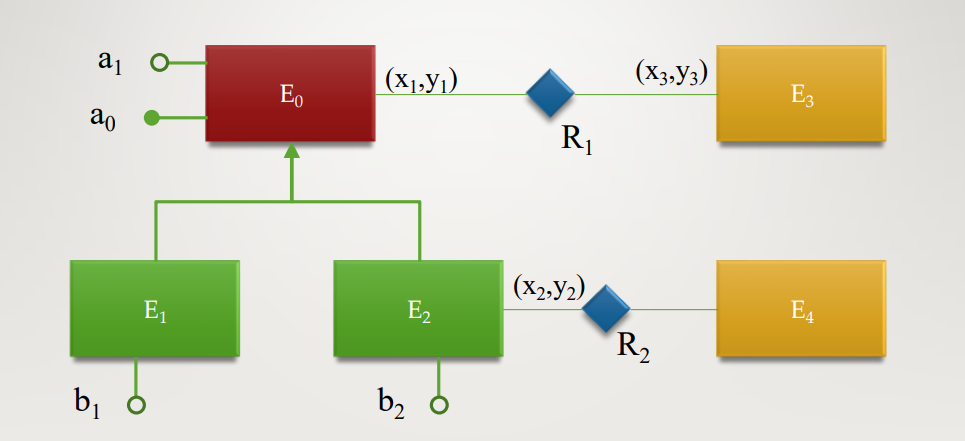
\includegraphics[width=1\linewidth]{image38.png}
    \caption{Schema iniziale}
\end{figure}

\begin{figure}[H]
    \centering
    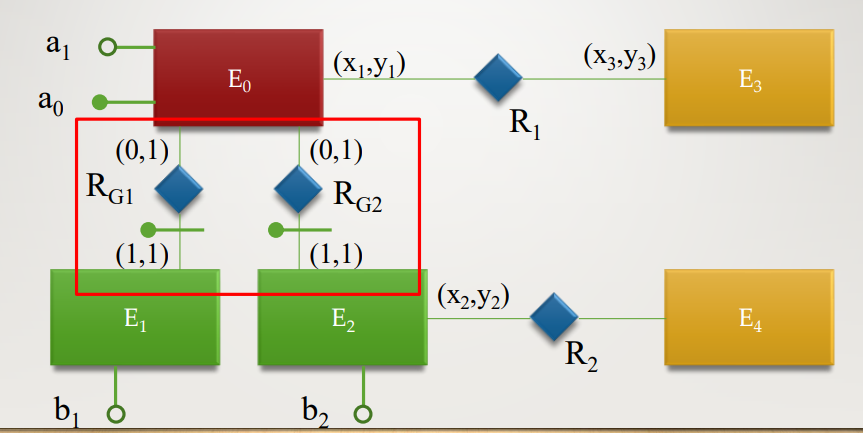
\includegraphics[width=1\linewidth]{image39.png}
    \caption{Sostituzione della generalizzazione con relazioni}
\end{figure}
\subsection{Traduzione verso il modello relazionale}

La traduzione verso il modello relazionale è un processo automatico che applica allo \textbf{schema concettuale ristrutturato} un insieme di regole di trasformazione.  
Ogni regola si applica a uno specifico costrutto del modello concettuale ER e produce una o più strutture del modello relazionale.

I principi fondamentali della traduzione sono:
\begin{itemize}
    \item Un’\textbf{istanza di entità} viene rappresentata mediante una \textbf{tupla} della tabella che implementa l’entità.
    \item Un’\textbf{istanza di relazione} viene rappresentata tramite:
    \begin{itemize}
        \item un \textbf{legame tra tuple} (mediante chiavi esterne), oppure
        \item una \textbf{tupla esplicita} in una tabella dedicata.
    \end{itemize}
    \item L’\textbf{identificatore principale} di un’entità viene rappresentato come \textbf{chiave primaria} della tabella che implementa tale entità.
\end{itemize}
\subsection{Classificazione delle relazioni binarie}

Una relazione binaria del modello ER può assumere tre forme, in base alle \textbf{cardinalità massime} delle entità coinvolte:

\begin{itemize}
    \item \textbf{Uno a Uno (1:1)}:  
    entrambe le entità coinvolte nella relazione hanno cardinalità massima pari a 1.

    \item \textbf{Uno a Molti (1:N)}:  
    una delle entità ha cardinalità massima pari a 1, mentre l’altra ha cardinalità massima maggiore di 1.

    \item \textbf{Molti a Molti (N:M)}:  
    entrambe le entità hanno cardinalità massima maggiore di 1.
\end{itemize}
\subsection{Regole di traduzione}
\begin{figure}[H]
    \centering
    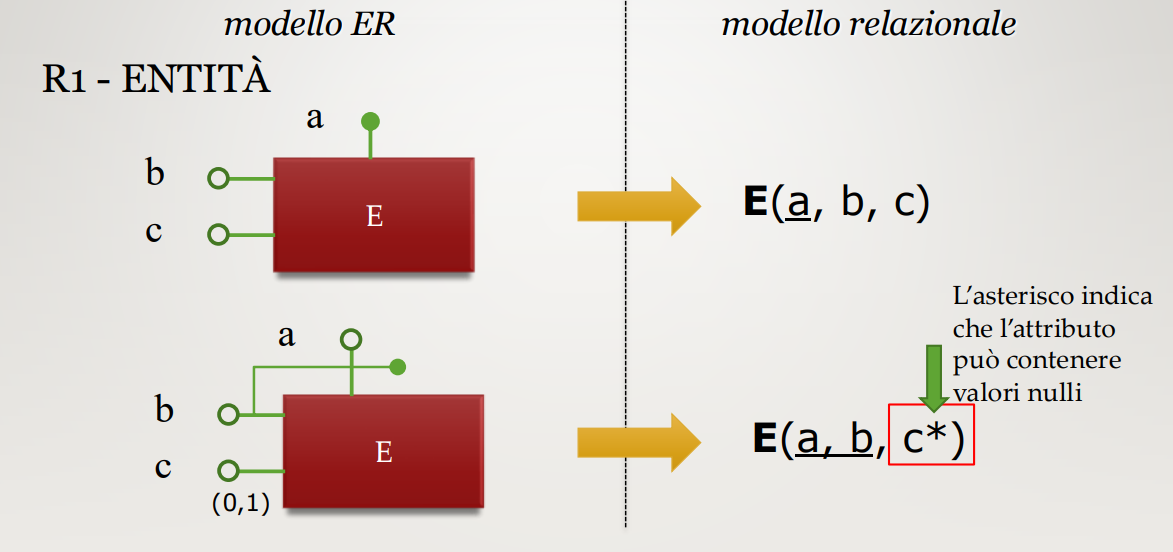
\includegraphics[width=1\linewidth]{image40.png}
    \caption{Entità}
\end{figure}
\begin{figure}[H]
    \centering
    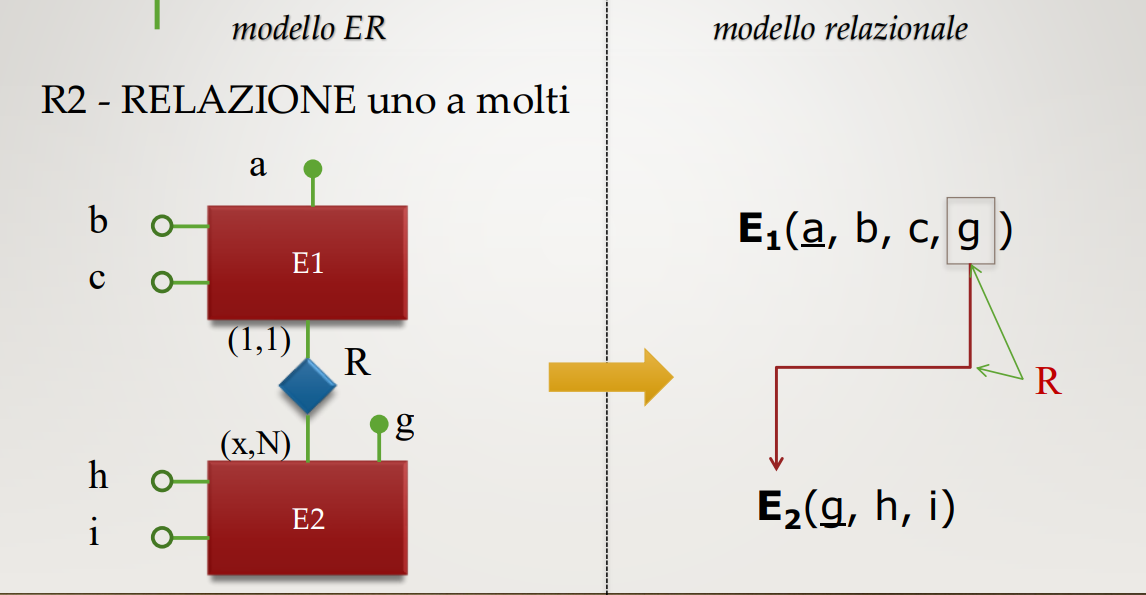
\includegraphics[width=1\linewidth]{image41.png}
    \caption{Relazione uno a molti}
\end{figure}
\begin{figure}[H]
    \centering
    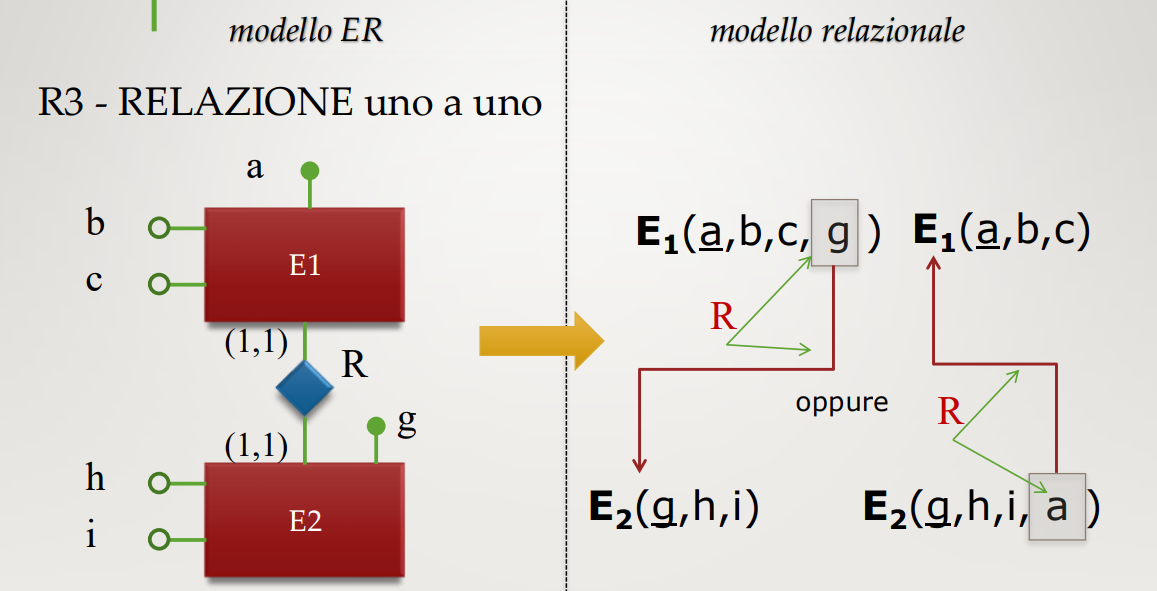
\includegraphics[width=1\linewidth]{image42.png}
    \caption{Relazione uno a uno}
\end{figure}
\begin{figure}[H]
    \centering
    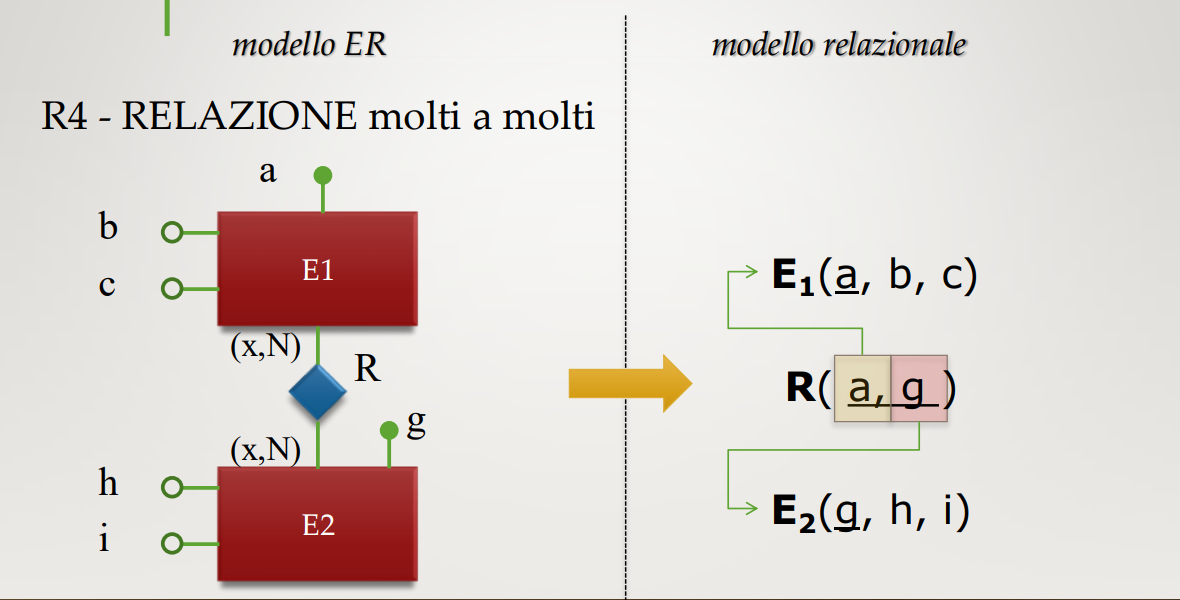
\includegraphics[width=1\linewidth]{image43.png}
    \caption{Relazione molti a molti}
\end{figure}
\begin{figure}[H]
    \centering
    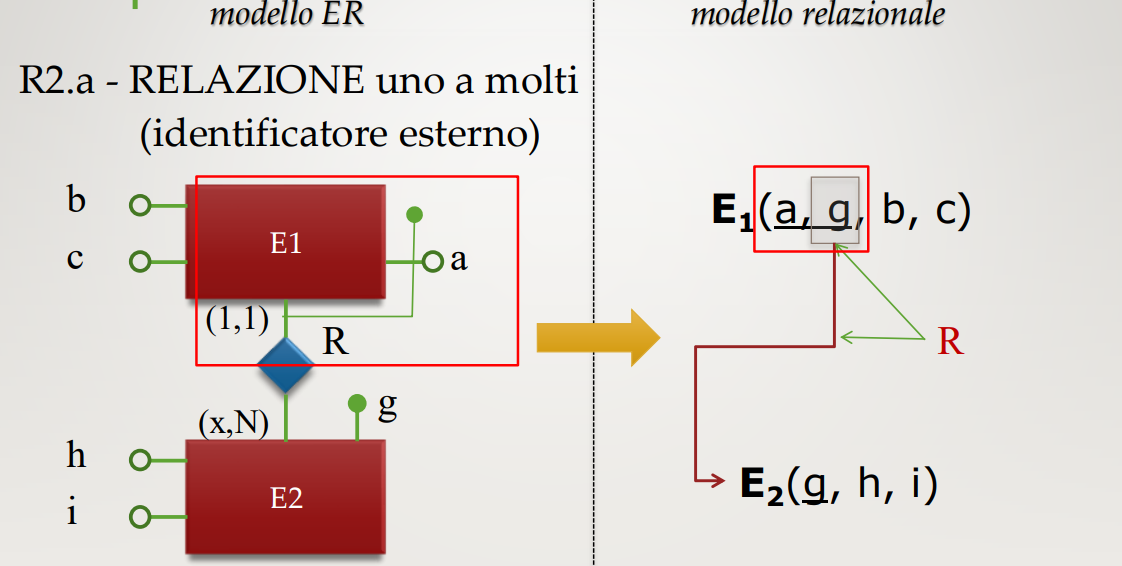
\includegraphics[width=1\linewidth]{image44.png}
    \caption{Relazione uno a molti identificatore esterno}
\end{figure}
\begin{figure}[H]
    \centering
    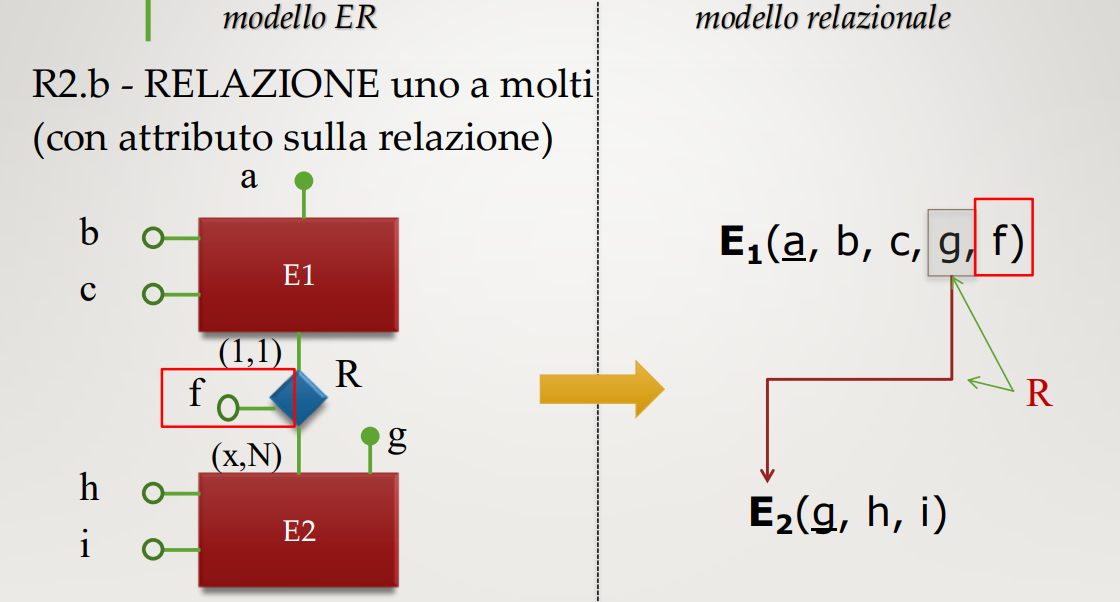
\includegraphics[width=1\linewidth]{image45.png}
    \caption{Relazione uno a molti con attributo sulla relazione}
\end{figure}
\begin{figure}[H]
    \centering
    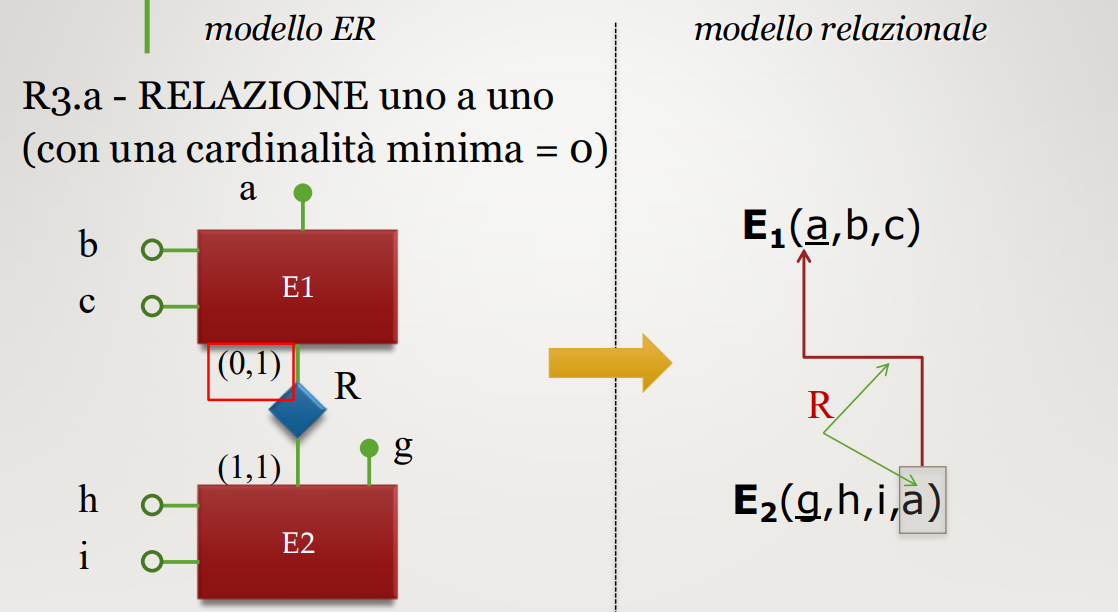
\includegraphics[width=1\linewidth]{image46.png}
    \caption{RELAZIONE uno a uno
(con una cardinalità minima = 0)}
\end{figure}
\begin{figure}[H]
    \centering
    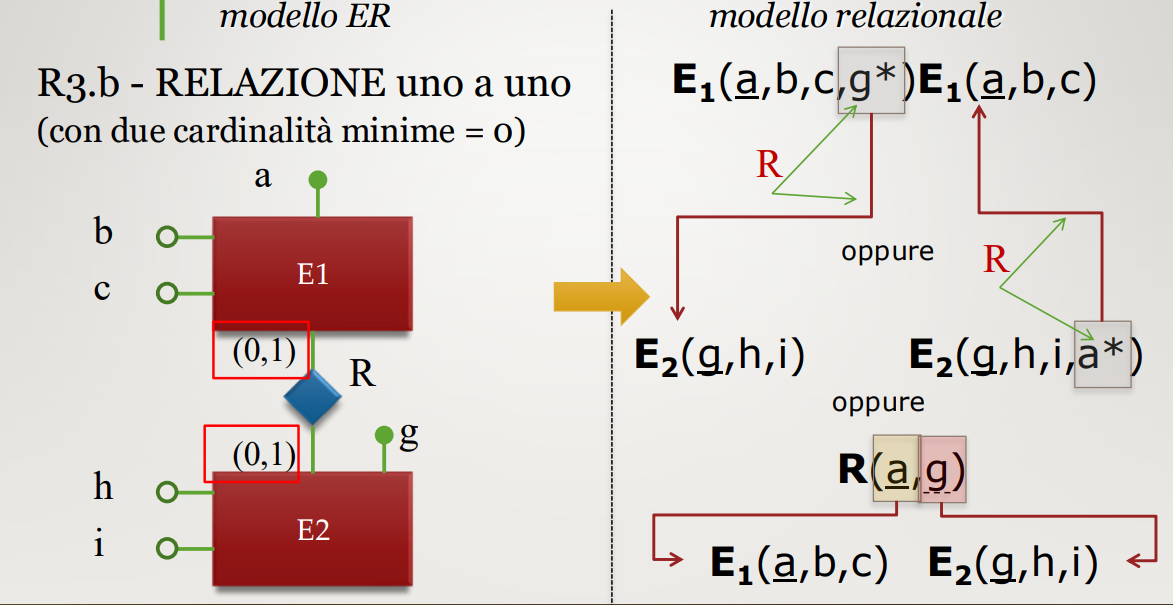
\includegraphics[width=1\linewidth]{image47.png}
    \caption{RELAZIONE uno a uno
(con due cardinalità minime = 0)}
\end{figure}
\begin{figure}[H]
    \centering
    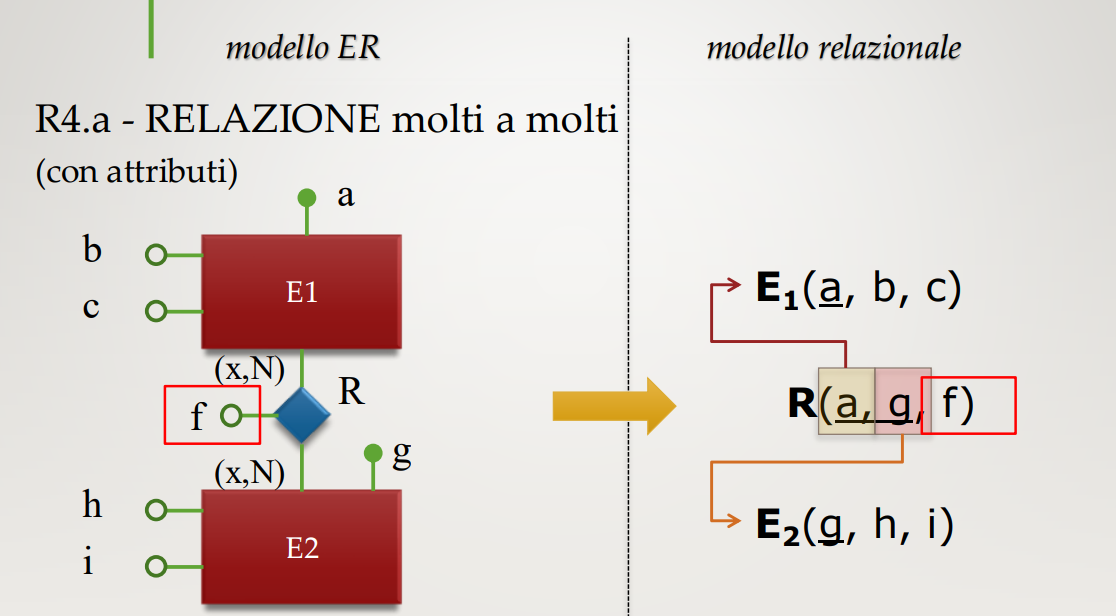
\includegraphics[width=1\linewidth]{image48.png}
    \caption{ - RELAZIONE molti a molti
(con attributi)}
\end{figure}
\begin{figure}[H]
    \centering
    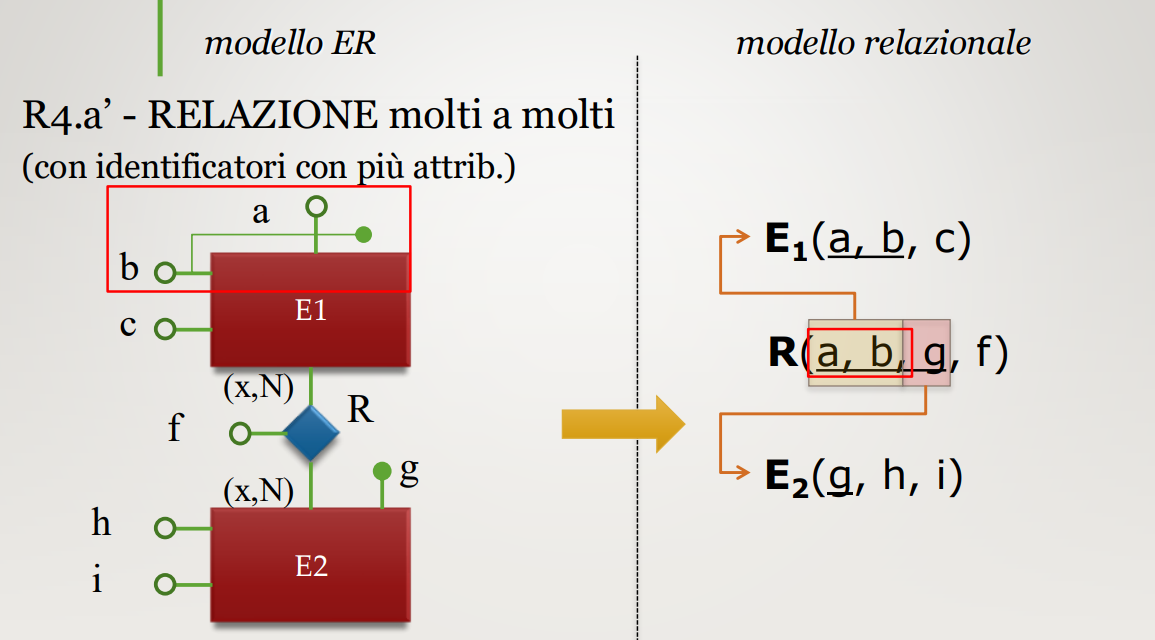
\includegraphics[width=1\linewidth]{image49.png}
    \caption{RELAZIONE molti a molti
(con identificatori con più attrib.) }
\end{figure}
\begin{figure}[H]
    \centering
    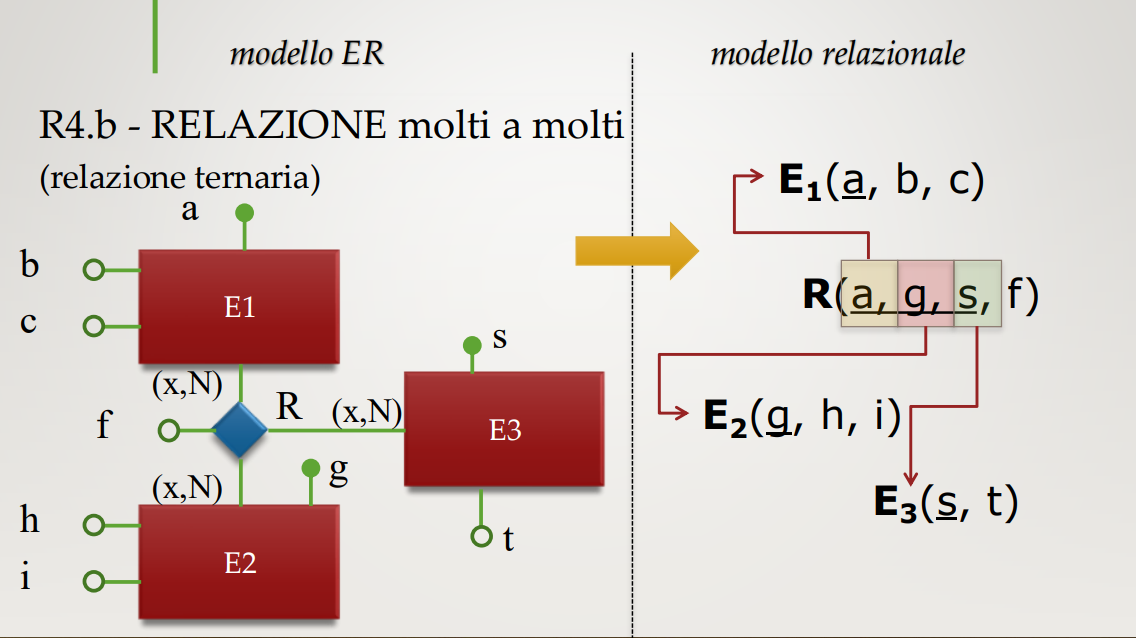
\includegraphics[width=1\linewidth]{image50.png}
    \caption{RELAZIONE molti a molti
(relazione ternaria)
}
\end{figure}
\begin{figure}[H]
    \centering
    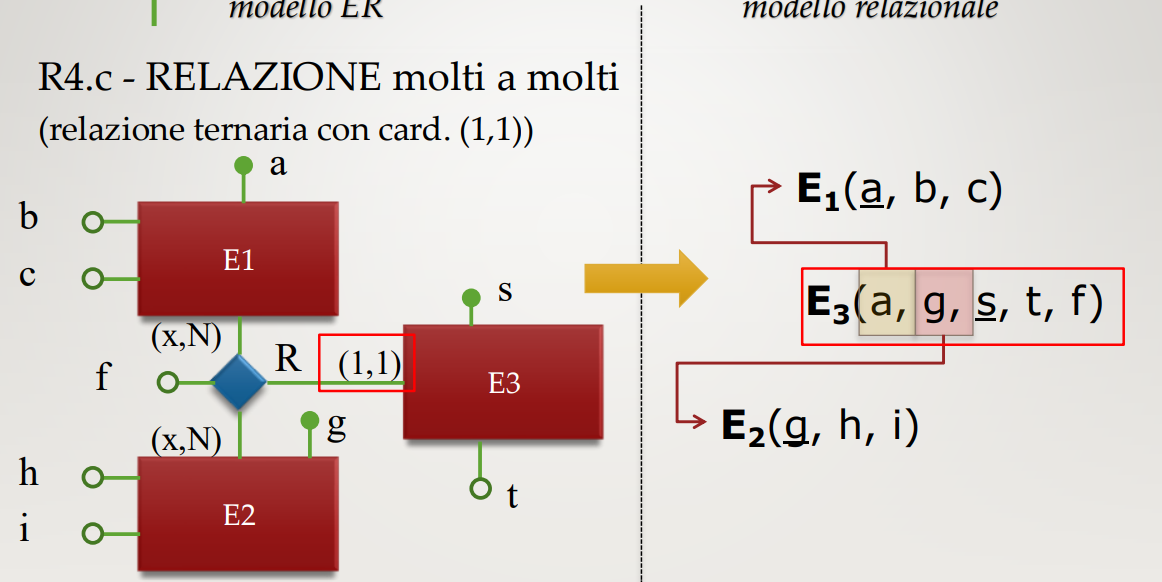
\includegraphics[width=1\linewidth]{image51.png}
    \caption{RELAZIONE molti a molti
(relazione ternaria con card. (1,1))}
    \label{fig:placeholder}
\end{figure}